\section{Mechanical analysis}
\subsection{Reference frames}
In order to study the behavior of the robot we will use the following frames:
\begin{itemize}
    \item Absolute frame: From a fix object in the room. 
    \item Body frame: From the body of our robot.
\end{itemize}

\begin{tikzpicture}[]
    \node (left_wheel) [cylinder, shape border rotate=0, draw, minimum height=1mm, minimum width=15mm] {};

    \node (right_wheel) [cylinder, shape border rotate=0, draw, minimum height=1mm, minimum width=15mm] {};

    \coordinate (left_wheel 0 0);
    \coordinate (right_wheel 10 0);
\end{tikzpicture}


\subsection{Inclination control}
In order to keep the inclination at a certain angle $\phi$ we must be able to compensate all the torque being to the body.

\[\ddot{\phi} * I_{body} = \tau_{body} \]

Assuming that the body is well balanced and neglecting the torque generated by the friction with air, the sum of all the torques in the motor axis applied to the body is equal to the sum of the torque applied by the motors:

\[\tau_{body} = \sum \tau_{motors}\]

The torque that the motors deliver to the wheels and to the flywheel create a reaction in the body in the opposite direction.


\[\tau_{body} = -\tau_{right-wheel} -\tau_{left-wheel} -\tau_{flywheel} \]

If we want to control the inclination $\phi$, we must be able to control $\tau_{body}$ in a range $\tau_{body} \in (-\epsilon, \epsilon)$. Observe that the angular acceleration $\ddot{\phi}$ of the body is linearly dependent with the torque it receives. In order to simplify the calculations we will assume $\epsilon = 0$.

\begin{equation} \label{eq:control equation}
0 = -\tau_{right-wheel} -\tau_{left-wheel} -\tau_{flywheel} \Rightarrow \tau_{right-wheel} +\tau_{left-wheel} = -\tau_{flywheel}
\end{equation}
In other words, we must compensate the torque of the wheels with the torque of the flywheel.

\subsection{Wheels torque}
The wheel torque we can induce is limited by the motor specifications. Note that the maximum torque of the motor is a function of velocity and in particular at max speed the torque is zero.

\[\tau_{motor} (w_{wheel}) \]


We assume that the wheels just roll and do no slip.
The robot is pushed by the wheels that make a force $F_{drag}$ against the ground in the contact point. See figure \ref{fig:Wheel force diagram}.

We can express the torque at the center of the of the wheel as:
\[\tau_{wheel} - F_{drag} * r_{wheel} = I_{wheel} * \dot{w}_{wheel} \]

\begin{equation} \label{wheel torque equation}
\tau_{wheel} = min(\tau_{motor} (w_{wheel}),I_{wheel} * \dot{w}_{wheel} + F_{drag} * r_{wheel})
\end{equation}
\begin{figure}[ht]
	\centering
	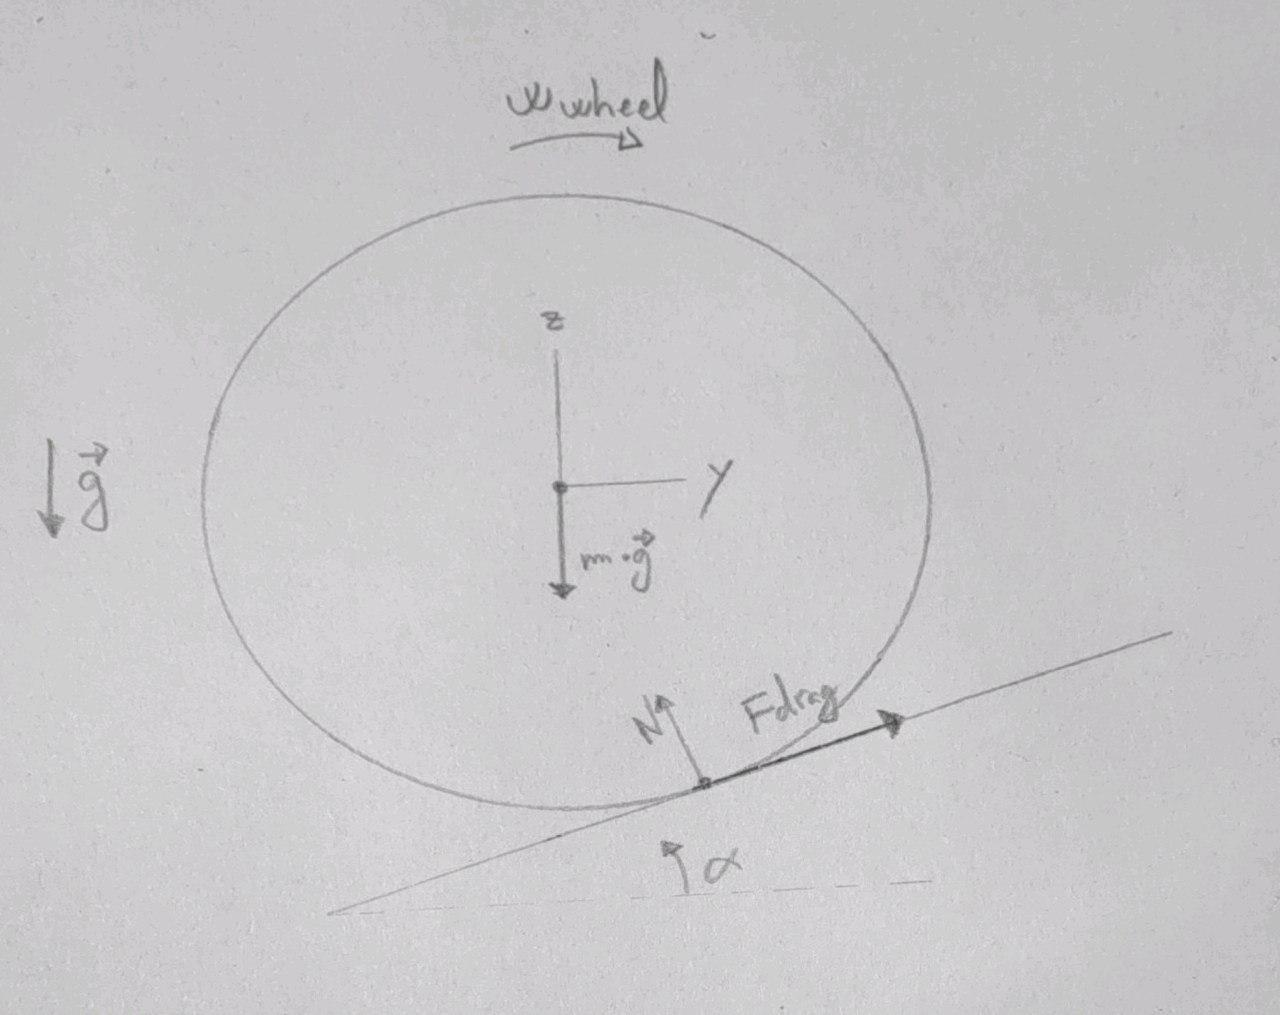
\includegraphics[width=10cm]{img/wheel_diagram.jpg}
	\caption{Wheel force diagram}
	\label{fig:Wheel force diagram}
\end{figure}


\subsection{Flywheel torque}

\begin{figure}
	\centering
	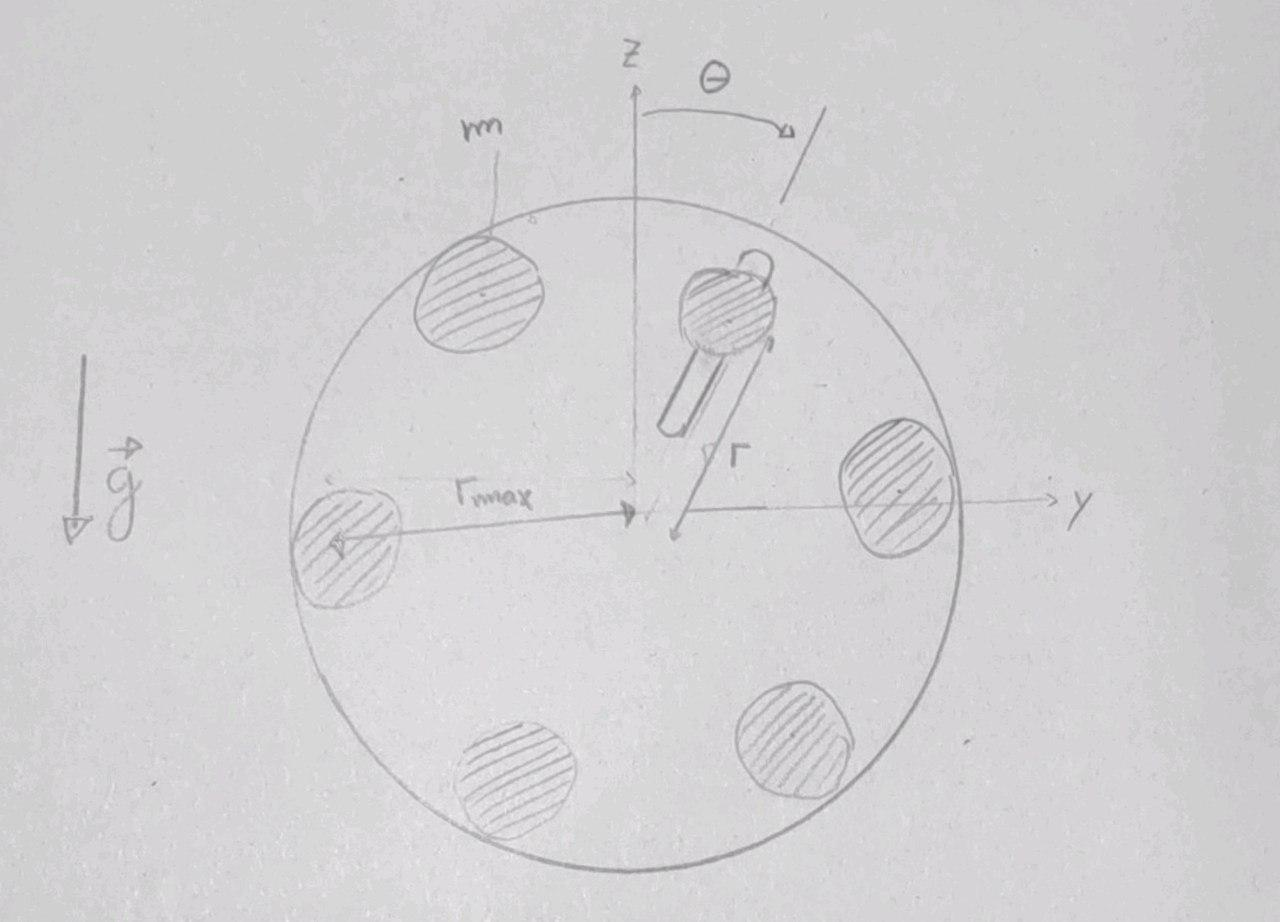
\includegraphics[width=10cm]{img/flywheel_diagram.jpg}
	\caption{Flywheel force diagram}
	\label{fig:Flywheel force diagram}
\end{figure}

The flywheel torque we can induce is also limited by the motor specifications. 

Assuming a general configuration of the flywheel where the moving mass is at distance $r$ and angle $\theta$, see figure \ref{fig:Flywheel force diagram}. we formulate its torque the following way:

\begin{equation}\label{flywheel equation}
    \tau_{flywheel} = min(\tau_{motor} (w), \ddot{\theta}*I_{flywheel}(r) + m_{cylinder} * g * (r - r_{max}) * \sin{\theta})  
\end{equation}

\subsection{Maximum speed and acceleration}
\begin{figure}
	\centering
	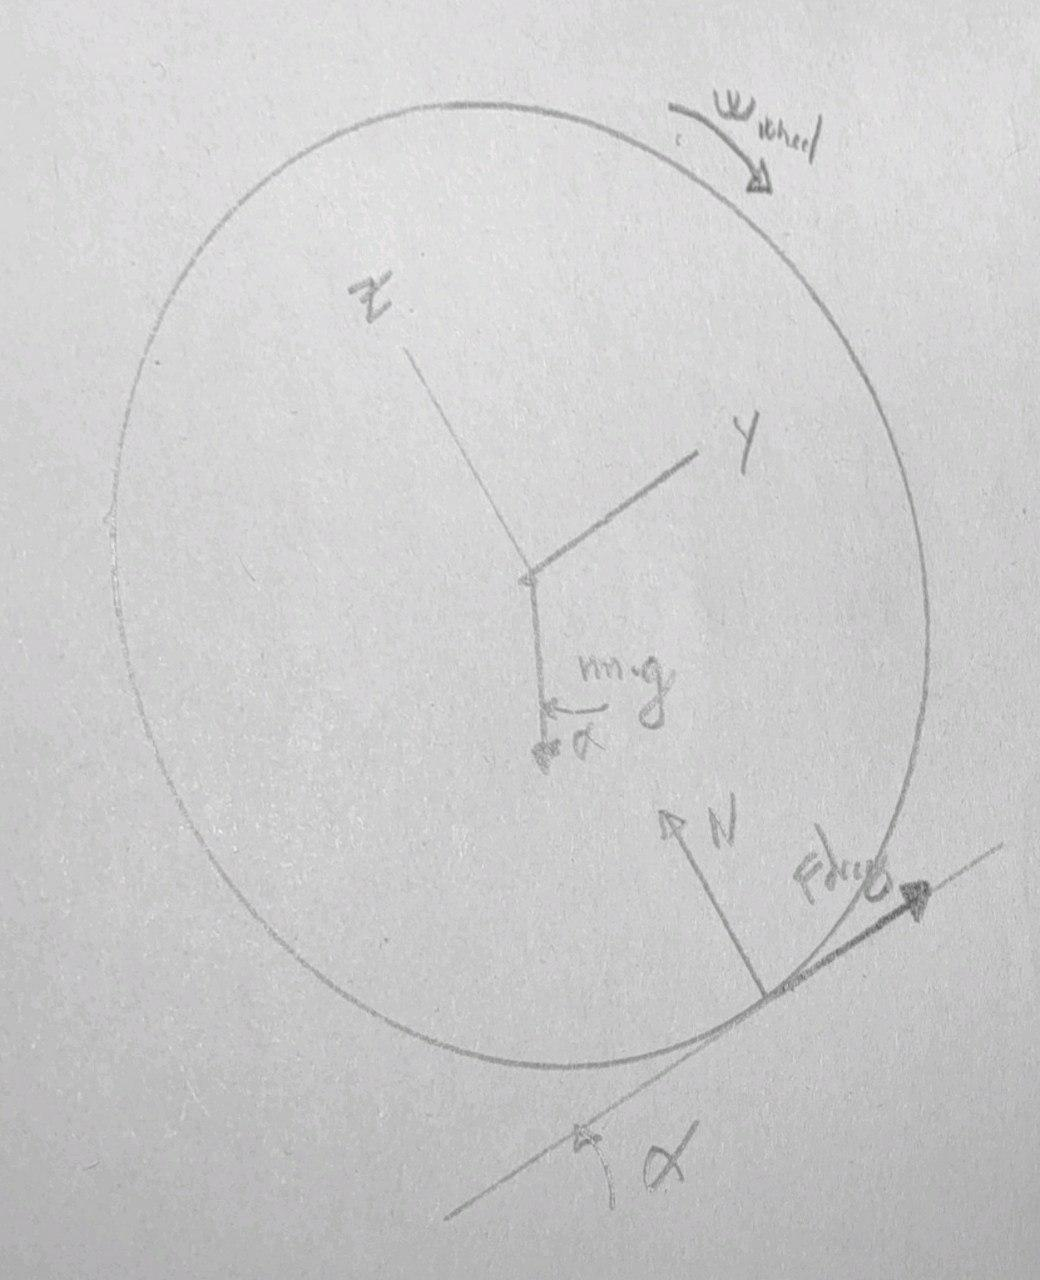
\includegraphics[width=10cm]{img/wheel_diagram_drag.jpg}
	\caption{Wheel force diagram}
	\label{fig:Wheel forward force diagram}
\end{figure}
We will assume both wheels turn at the same speed, have the same $F_{drag}$ and the same $\tau_{wheel}$:
\[ w_{wheel-left} = w_{wheel-right} = w \]

Applying Newton's first law in the y axis of figure \ref{fig:Wheel forward force diagram}
\[\ddot{y}*m_{total} = 2 * F_{drag} - m_{total} * g * sin(\alpha)\]

Substituting $F_{drag}$ taking in to account equation \ref{wheel torque equation}:
\[\ddot{y}*m_{total} = 2 * \frac{\tau_{wheel} - I_{wheel} * \dot{w}_{wheel}}{r_{wheel}} - m_{total} * g * sin(\alpha)\]

Using equation \ref{eq:control equation}:
\begin{equation}\label{eq of acceleration}
    \Rightarrow  \ddot{y}*m_{total} = - \frac{\tau_{flywheel}}{r_{wheel}} - \frac{I_{wheel} * \dot{w}_{wheel}}{r_{wheel}} - m_{total} * g * sin(\alpha)
\end{equation}


We will now study different cases to better understand this equation.
\subsubsection{No terrain inclination ($\alpha = 0$)}
The equation we get is substituting $\alpha = 0$ in equation \ref{eq of acceleration}:
\[\ddot{y}*m_{total} = - \frac{\tau_{flywheel}}{r_{wheel}} - \frac{I_{wheel} * \dot{w}_{wheel}}{r_{wheel}}\]

Substituting equation \ref{flywheel equation}
\begin{equation}\label{no inclintation eq}
    \ddot{y}*m_{total} = - \frac{\ddot{\theta}*I_{flywheel}(r) + m_{cylinder} * g * (r - r_{max}) * \sin{\theta}}{r_{wheel}} - \frac{I_{wheel} * \dot{w}_{wheel}}{r_{wheel}}
\end{equation}


We will now split the study in  three cases:
\begin{enumerate}
    \item Flywheel case: $r$ is fixed to $r = r_{max}$ 
    
    Then:  
    \[\ddot{y}*m_{total} = - \frac{\ddot{\theta}*I_{flywheel}(r_{max})}{r_{wheel}} - \frac{I_{wheel} * \dot{w}_{wheel}}{r_{wheel}}\]

    Taking in two account the following relation:
    \[w_{wheel} * r_{wheel} = \dot{y} \Rightarrow  \dot{w}_{wheel} * r_{wheel} = \ddot{y} \]

    The moment of inertia are:
    \[I_{wheel} = \frac{1}{2} *m_{wheel} * r_{wheel}^2\]
    \[I_{flywheel} \approx 6 * m_{cylinder} * r_{max}^2\]

    Let's go for it:
    \[\dot{w}_{wheel} * r_{wheel}*m_{total} = - \frac{\ddot{\theta}*6 * m_{cylinder} * r_{max}^2}{r_{wheel}} - \frac{1}{2} *m_{wheel} * r_{wheel} * \dot{w}_{wheel} \]

    \[\dot{w}_{wheel} * r_{wheel}*(m_{total}+\frac{1}{2} *m_{wheel}) = - \frac{\ddot{\theta}*6 * m_{cylinder} * r_{max}^2}{r_{wheel}}\]


    We define R as the quotient between $\dot{w}_{wheel}$ and $-\ddot{\theta}$

    \[R = \frac{\dot{w}_{wheel}}{-\ddot{\theta}} = \frac{6 * m_{cylinder} * r_{max}^2}{(m_{total} + \frac{1}{2} *m_{wheel}) * r_{wheel}^2} \]

    We can see that R will always be smaller than 1 because $6 * m_{cylinder} < m_{total} $ and $r_{max} < r_{wheel}$. This means that we will be limited by the acceleration of the flywheel.

    The forward acceleration is:
    \[\ddot{y} = \dot{w}_{wheel} * r_{wheel} = - R * \ddot{\theta} * r_{wheel}\]

    And using equation \ref{flywheel equation} we get that the maximum is:

    \[\tau_{motor} (w) = \ddot{\theta}*I_{flywheel}(r) \Rightarrow \ddot{\theta} = \frac{\tau_{motor} (\dot{\theta})}{I_{flywheel}(r)} \]

    \[\ddot{y}_{max} = - R * \frac{\tau_{motor} (\dot{\theta})}{I_{flywheel}(r)} * r_{wheel}\]

    \[\Rightarrow \ddot{y}_{max} = -\frac{6 * m_{cylinder} * r_{max}^2}{(m_{total} + \frac{1}{2} *m_{wheel}) * r_{wheel}^2} * \frac{\tau_{motor} (\dot{\theta})}{I_{flywheel}(r)} * r_{wheel}\]
    
    \[\boxed{\Rightarrow \ddot{y}_{max} = -\frac{\tau_{motor} (\dot{\theta})}{(m_{total} + \frac{1}{2} *m_{wheel}) * r_{wheel}}} \]
    
    In order to compute the maximum speed we will assume that the initial conditions are $\dot{\theta} = 0$ and $w_{wheel-max}=0$

    \[w_{wheel-max} = \int_{w_{wheel-0}}^{w_{wheel-max}} \dot{w}_{wheel} dt\]

    Now we will proceed to do a change of variables in the integral.
    
    \[\ddot{\theta} = -\frac{\dot{w}_{wheel}}{R}\]
    \[\Rightarrow \dot{w}_{wheel} = - \ddot{\theta} * R \] 

    \[w_{wheel-max} = -R * \int_{\dot{\theta}_0}^{\dot{\theta}_{max}} \ddot{\theta} *   dt = -R * \dot{\theta}_{max}\]

    \[\boxed{\dot{y}_{max} = - r_{wheel} * R * \dot{\theta}_{max}}\]

    And $\dot{\theta}_{max}$ is a limitation imposed by the motor specifications.




    \item Pendulum: $\dot{\theta} = 0$, and $r$ is fixed to $r = r_{min}$
    
    Using equation \ref{no inclintation eq} and $\ddot{\theta} = 0$
    \[\ddot{y}*m_{total} = - \frac{m_{cylinder} * g * (r - r_{max}) * \sin{\theta}}{r_{wheel}} - \frac{I_{wheel} * \dot{w}_{wheel}}{r_{wheel}}\]
    \[\ddot{y}*m_{total} * r_{wheel} = - m_{cylinder} * g * (r - r_{max}) * \sin{\theta} - I_{wheel} * \dot{w}_{wheel}\]
    And $\dot{w}_{wheel} = \frac{\ddot{y}}{r_{wheel}}$
    \[\ddot{y}*m_{total} * r_{wheel} + I_{wheel} * \frac{\ddot{y}}{r_{wheel}} = - m_{cylinder} * g * (r - r_{max}) * \sin{\theta} \]

    \[\ddot{y}  = -\frac{m_{cylinder} * g * (r - r_{max}) * \sin{\theta}}{m_{total} * r_{wheel} + \frac{I_{wheel}}{r_{wheel}} }  \]
    Replacing $I_{wheel}$ and $r=r_{min}$
    \[\ddot{y}  = -\frac{m_{cylinder} * g * (r_{min} - r_{max}) * \sin{\theta}}{ r_{wheel} * (m_{total} + \frac{1}{2} * m_{wheel}) }  \]

    Which is maximum when $\sin{\theta}=1$
    \[\boxed{\ddot{y}_{max}  = \frac{m_{cylinder} * g * (r_{max}- r_{min})}{ r_{wheel} * (m_{total} + \frac{1}{2} * m_{wheel}) } } \]
    
    And there is no limitation on the maximum speed.

    \item We leave the weight free:
    
    TO DO: ODE    
\end{enumerate}

\subsubsection{No acceleration, just inclination ($\alpha > 0$)}
Substituting $\ddot{y}=0$ in equation \ref{eq of acceleration}
\[m_{total} * g * sin(\alpha) = - \frac{\tau_{flywheel}}{r_{wheel}} \]
\[sin(\alpha) = - \frac{\tau_{flywheel}}{m_{total} * g * r_{wheel}} \]

We are going to distinguish the same three cases as before:
\begin{enumerate}
    \item Flywheel case: $r$ is fixed to $r = r_{max}$
    Substituting equation \ref{flywheel equation}
    \[sin(\alpha) = - \frac{min(\tau_{motor} (w), \ddot{\theta}*I_{flywheel}(r))}{m_{total} * g * r_{wheel}} \]
    The maximum inclination at a certain moment:
    \[sin(\alpha_{max}) = - \frac{\tau_{motor} (w)}{m_{total} * g * r_{wheel}} \]
    Maximum height can that the robot can achieve under the initial conditions $\dot{y}=\dot{y}_0$ and $\dot{\theta}=\dot{\theta}_0$:
    \[h_{max}=\int_{\dot{\theta}_0}^{\dot{\theta}_{max}} \dot{y}_0*sin(\alpha) * dt  = \dot{y}_0* \int_{\dot{\theta}_0}^{\dot{\theta}_{max}} - \frac{\ddot{\theta}*I_{flywheel}(r)}{m_{total} * g * r_{wheel}} * dt\]
    \[\boxed{\Rightarrow h_{max}= \dot{y}_0* (\dot{\theta}_0-\dot{\theta}_{max}) * \frac{I_{flywheel}(r)}{m_{total} * g * r_{wheel}}}\]

    \item Pendulum: $\dot{\theta} = 0$, and $r$ is fixed to $r = r_{min}$
    \[sin(\alpha) = - \frac{m_{cylinder} * g * (r - r_{max}) * \sin{\theta}}{m_{total} * g * r_{wheel}} = \frac{m_{cylinder} * (r_{max}- r_{min}) * \sin{\theta}}{m_{total} * r_{wheel}} \]
    \[sin(\alpha_{max}) = - \frac{m_{cylinder} * g * (r - r_{max}) * \sin{\theta}}{m_{total} * g * r_{wheel}}\]
    \[\boxed{sin(\alpha_{max}) = \frac{m_{cylinder} * (r_{max}- r_{min}) * \sin{\theta}}{m_{total} * r_{wheel}}} \]
    
    \item We leave the weight free:
    ODE

\end{enumerate}
\subsection{Shear stress}
The shear strength $\tau_{shear}$


\subsection{Motor specifications}

Here we have the factory specifications of our motors: 
\begin{itemize}
    \item Operating voltage: between 3 V and 9 V
    \item Nominal voltage: 6 V
    \item Free-run speed at 6 V: 176 RPM
    \item Free-run current at 6 V: 80 mA
    \item Stall current at 6V: 900 mA
    \item Stall torque at 6V: 5 kg·cm
    \item Gear ratio: 1:35
    \item Reductor size: 21 mm
    \item Weight: 85 g
\end{itemize}

\subsection{Hypothesis}
Assuming that the body is well balanced
